\documentclass[main.tex]{subfiles}

\begin{document}
\chapter{Parallelisation of electronic-structure calculations\label{ch:optimisation_scf}}

The \texttt{PWscf} (Plane-Wave Self-Consistend Field) package is one of the core modules of \QE, as many other modules need ground state density and total energy as input.
This chapter deals with examining the best ways to run \texttt{PWscf} calculations in the \texttt{scf} mode.

\section{First scaling tests}\label{sec:scf_first_scaling}

The first step in analysing the scaling of the \texttt{PWscf} module is to perform a baseline scaling test without any optimisations appplied. 
In Fig. \ref{fig:scaling_scf_ompi_nprocs_si_speedup} to \ref{fig:scaling_scf_ompi_nprocs_tas2_absolute_wait} two scaling tests on the earlier mentioned benchmarking systems Si and \TaS are pictured. 
The tests are run using \QE 7.0, compiled using the Fortran and C compilers in \gls{openmpi} 4.1.0, without any of the compilation or runtime optimisation parameters mentioned in section \ref{sec:qe} used.

\begin{figure}[ht!]
\centering
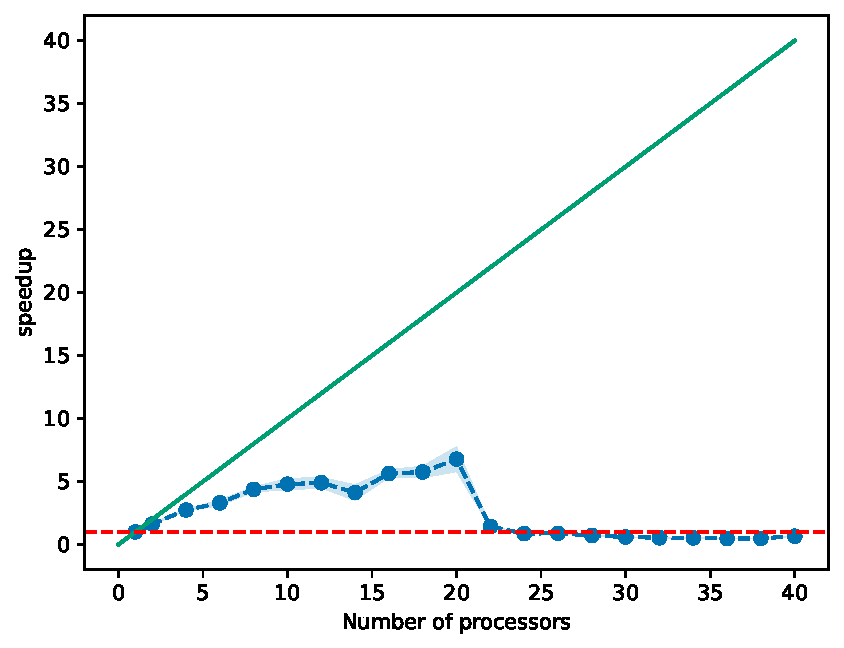
\includegraphics[width=0.75\textwidth]{plots_scf/si_ompi_bench_nprocs_speedup.pdf}
\caption{Scalability for the Si benchmarking system, \emph{\QE 7.0, \gls{openmpi} 4.1.0, \texttt{nk 1} and \texttt{nd 1}}}
\label{fig:scaling_scf_ompi_nprocs_si_speedup}
\end{figure}

\begin{figure}[ht!]
\begin{subfigure}[b]{0.49\textwidth}
    \centering
    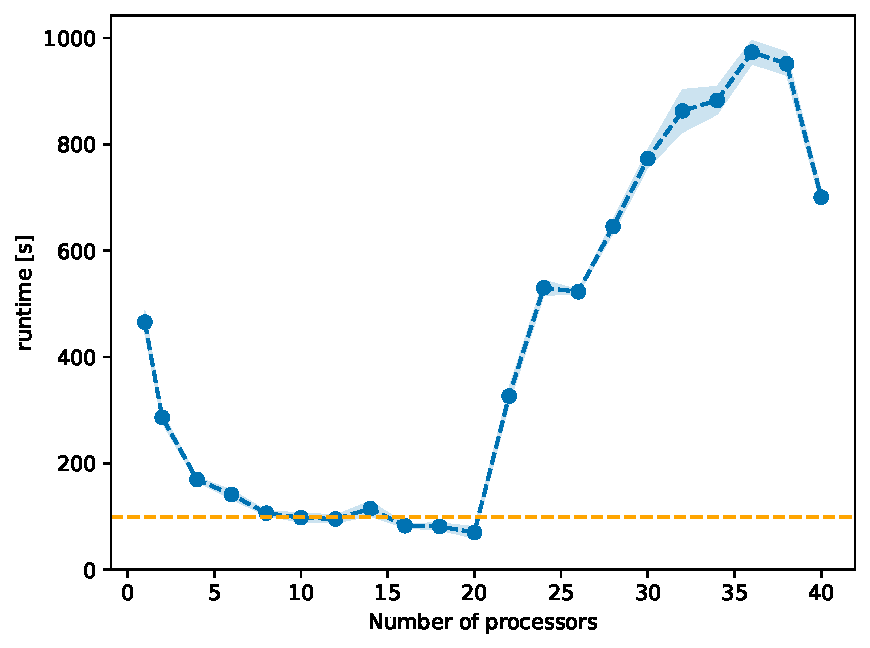
\includegraphics[width=\textwidth]{plots_scf/si_ompi_bench_nprocs_absolute.pdf}
\end{subfigure}
\begin{subfigure}[b]{0.49\textwidth}
    \centering
    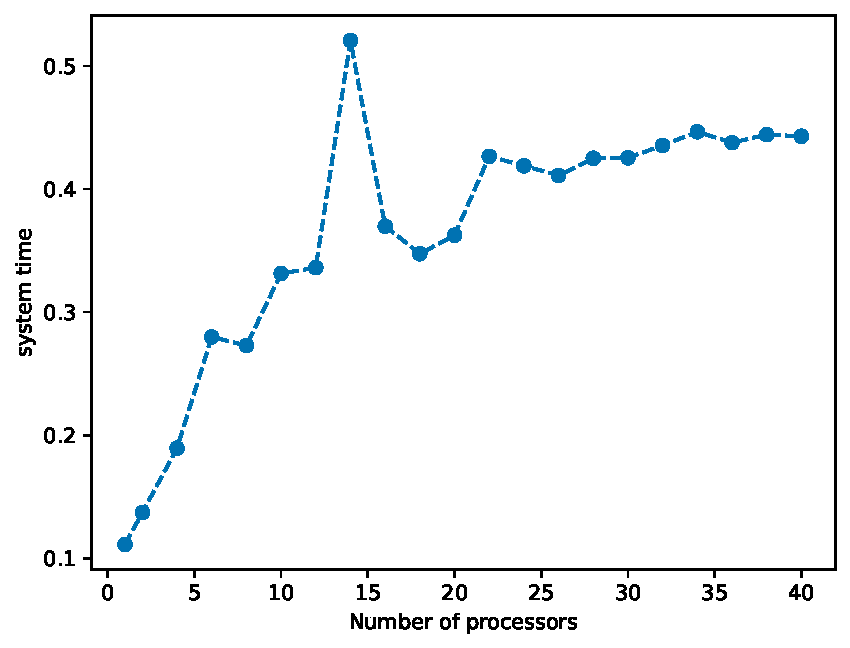
\includegraphics[width=\textwidth]{plots_scf/si_ompi_bench_nprocs_wait.pdf}
\end{subfigure}
\caption{Absolute runtime and wait time for the scalability test on the Si benchmarking system, \emph{\QE compiled with \gls{openmpi} 4.1.0, \texttt{nk 1} and \texttt{nd 1}}}
\label{fig:scaling_scf_ompi_nprocs_si_absolute_wait}
\end{figure}

As discussed in sec. \ref{sub:scalability_qe}, three different metrics of scalability can be deduced from the time data given by \QE:
\begin{itemize}
    \item runtime: absolute runtime (walltime) of the compute job
    \item speedup: runtime divided by runtime of the job on a single core
    \item \gls{wait_time}: percentage of \gls{wall_time} used by system tasks, e.g. writing to disk, etc.
\end{itemize}
These are pictured in fig. \ref{fig:scaling_scf_ompi_nprocs_si_speedup} and \ref{fig:scaling_scf_ompi_nprocs_si_absolute_wait} for the silicon benchmarking system.

On a single node, the speedup does scale linearly with the number of processors until around 10 processors, but with a slope of \(\frac{1}{2}\) instead of 1 (which would mean ideal scaling).
Beyond that number, the slope decreases even more so that a maximal speedup of around 7 is achieved for 20 processors used.
One compute node is equipped with 20 cores, so trying to scale the communication intensive calculations beyond that threshold makes the calculations run even slower than on a single core.
Interestingly, the wait time plot in \ref{fig:scaling_scf_ompi_nprocs_si_absolute_wait} shows that a significant amount (\(\SI{10}{\percent}\) to \(\SI{40}{\percent}\)) of runtime is taken up by wait time already for less than 20 processors.
As discussed in sec. \ref{sub:scalability_general}, this is a sign of poor parallelization, which can explain the poor scaling seen in fig. \ref{fig:scaling_scf_ompi_nprocs_si_speedup}.

Pictured in fig. \ref{fig:scaling_scf_ompi_nprocs_tas2_speedup} and \ref{fig:scaling_scf_ompi_nprocs_tas2_absolute_wait} are the same scaling test run for the \TaS benchmarking system.
Here, the speedup is not taken as runtime divided by runtime on a single core, as the memory required is more than what can be accessed by a single core.
Instead, an estimate of the single core runtime is made by multiplying the runtime of the job running on 4 cores by 4.
This assumes perfect scaling for 1-4 processors, but the relative scaling is accurate, no matter the accuracy of this assumption.

\begin{figure}[ht!]
\centering
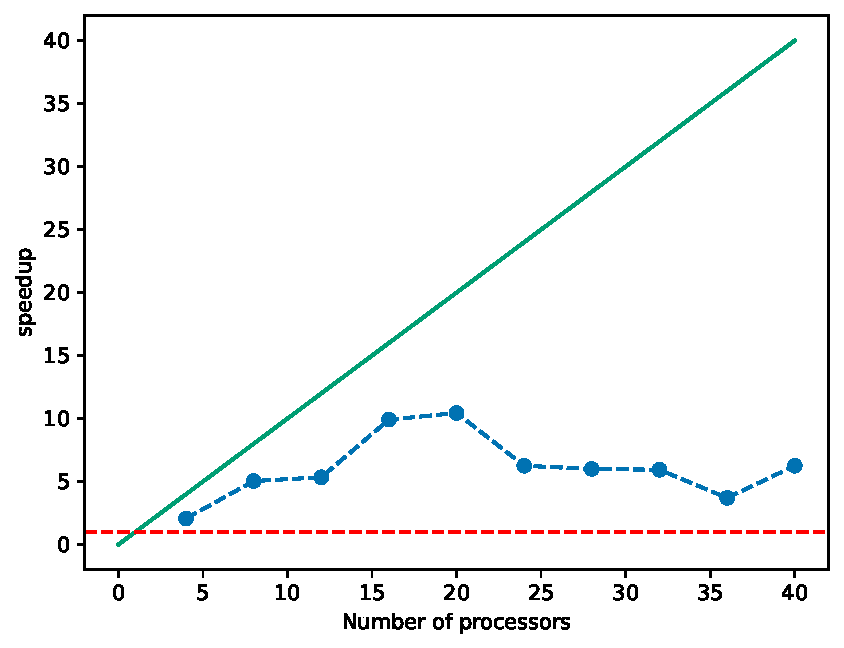
\includegraphics[width=0.75\textwidth]{plots_scf/TaS2_ompi_bench_nprocs_speedup.pdf}
\caption{Scalability for the \TaS benchmarking system, \emph{\QE 7.0, OpenMPI 4.1.0, \texttt{nk 1} and \texttt{nd 1}}}
\label{fig:scaling_scf_ompi_nprocs_tas2_speedup}
\end{figure}

\begin{figure}[ht!]
\begin{subfigure}[b]{0.49\textwidth}
    \centering
    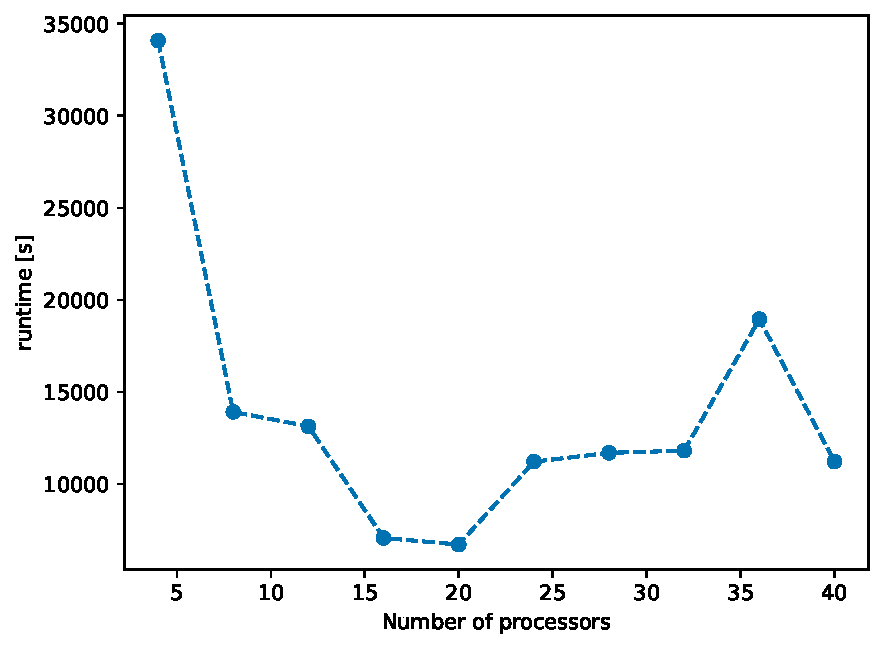
\includegraphics[width=\textwidth]{plots_scf/TaS2_ompi_bench_nprocs_absolute.pdf}
\end{subfigure}
\begin{subfigure}[b]{0.49\textwidth}
    \centering
    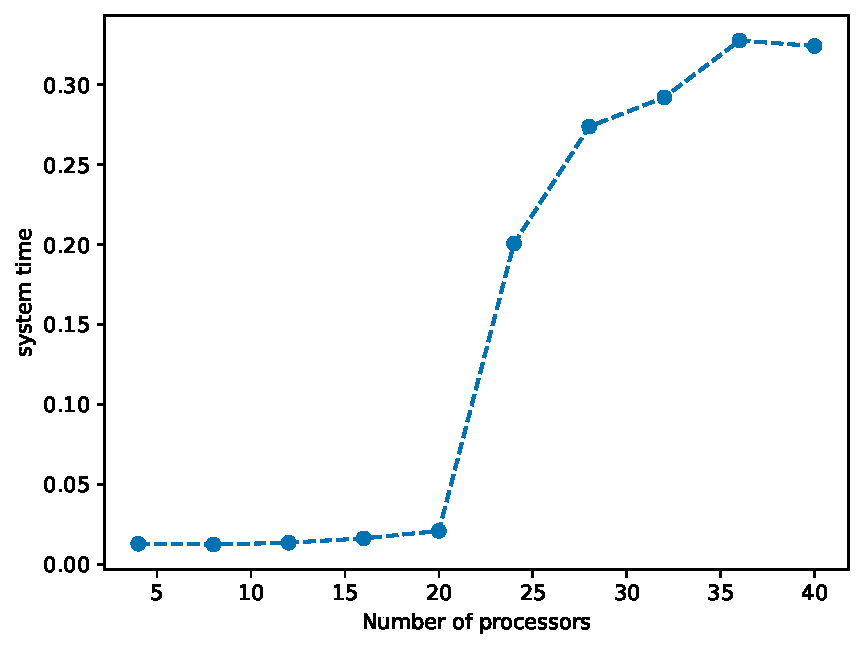
\includegraphics[width=\textwidth]{plots_scf/TaS2_ompi_bench_nprocs_wait.pdf}
\end{subfigure}
\caption{Absolute runtime and wait time for the scalability test on the \TaS benchmarking system, \emph{\QE 7.0, \gls{openmpi} 4.1.0, \texttt{nk 1} and \texttt{nd 1}}}
\label{fig:scaling_scf_ompi_nprocs_tas2_absolute_wait}
\end{figure}
The scaling test on the \TaS system shows much better scaling.
For up to 20 processors, the speedup follows the ideal scaling with a stark decline with more processors.
This is also reflected in the wait time in fig. \ref{fig:scaling_scf_ompi_nprocs_tas2_absolute_wait}, as it goes from a small constant value for under 20 processors to some kind of dependence of the number of processors, which hints to communication or bottlenecks being a limiting factor here.

In conclusion, systems with more electrons and by extension bigger matrices and longer iteration times seem to be parallelize better and as such profit more from using more processors than systems with just a few number of electrons.

These scaling tests now pose the question how better scaling over more than one node can be achieved.

\section{Testing different compilers and mathematical libraries}\label{sec:scf_scaling_compilers}

A first strategy for solving issues with parallelization is trying different compilers and mathematical libraries.
As discussed in sec. \ref{sub:qe_compilation}, \QE can make use of a variety of software packages available on the PHYSnet cluster.
The benchmarks in \ref{fig:scaling_scf_compilers_nprocs} are run with the following software combinations:
\begin{itemize}
    \item \gls{openmpi} 4.1.0 and \QE provided \gls{blas}/\gls{lapack}, so the baseline test discussed in sec. \ref{sec:scf_first_scaling}
    \item \gls{openmpi} 4.1.0, \gls{openblas} 0.3.20 and \gls{scalapack} 2.2.0
    \item \gls{oneapi} 2021.4
\end{itemize}

\begin{figure}[ht!]
\begin{subfigure}[b]{0.49\textwidth}
    \centering
    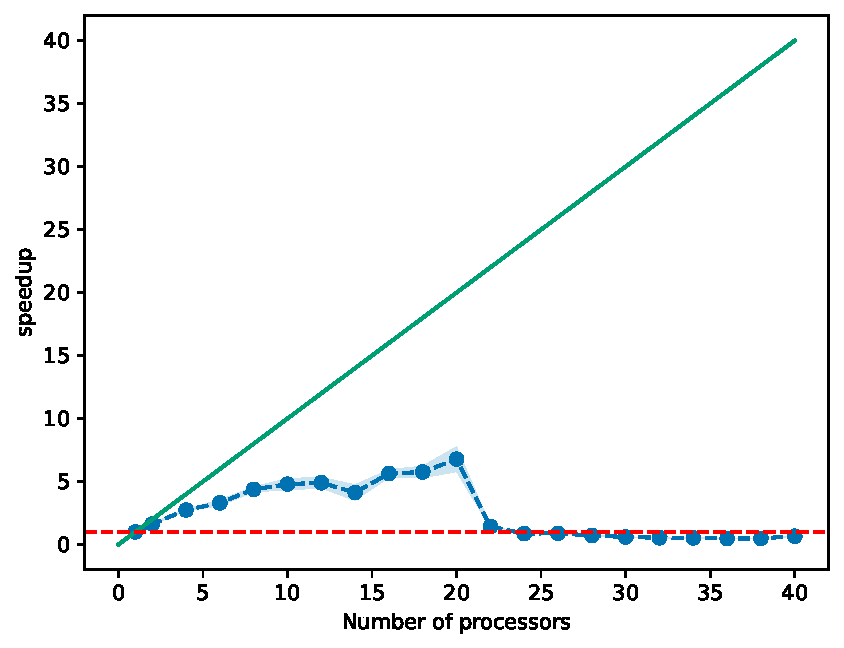
\includegraphics[width=\textwidth]{plots_scf/si_ompi_bench_nprocs_speedup.pdf}
    \subcaption{\gls{openmpi} 4.1.0}
\end{subfigure}
\begin{subfigure}[b]{0.49\textwidth}
    \centering
    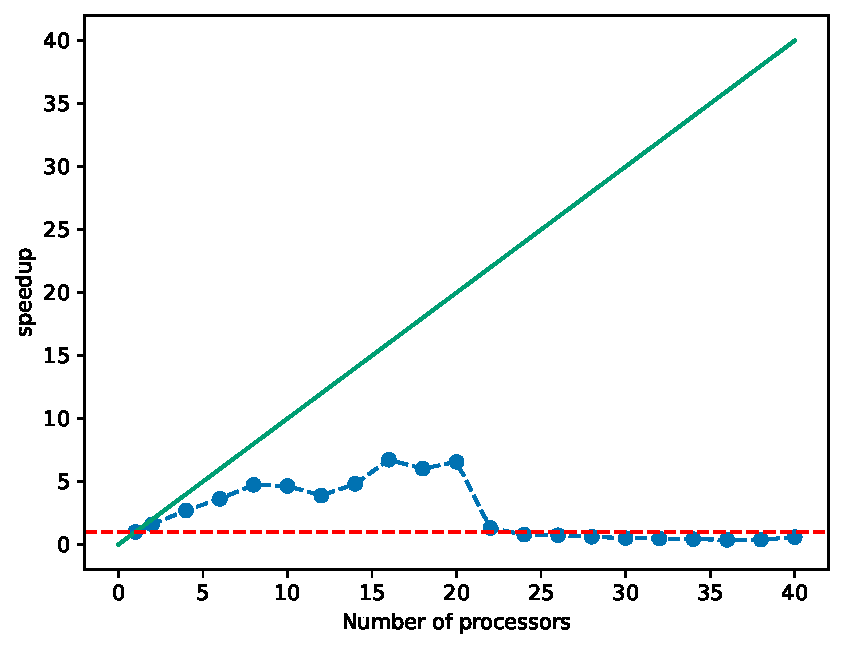
\includegraphics[width=\textwidth]{plots_scf/si_scalapack_bench_nprocs_speedup.pdf}
    \subcaption{\gls{openmpi} 4.1.0, \gls{openblas} 0.3.20, \gls{scalapack} 2.2.0}
\end{subfigure}
\begin{subfigure}[b]{0.49\textwidth}
    \centering
    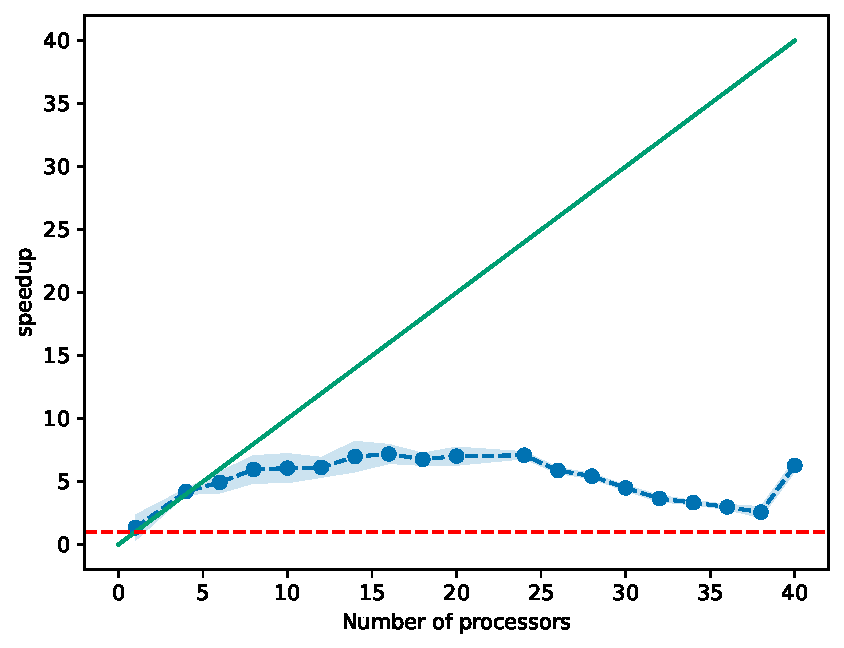
\includegraphics[width=\textwidth]{plots_scf/si_intel_bench_nprocs_speedup.pdf}
    \subcaption{\gls{oneapi} 2021.4}
\end{subfigure}
\caption{Scalability for the Si benchmarking system with different combinations of compilers and mathematical libraries, \emph{\texttt{nk 1} and \texttt{nd 1}}}
\label{fig:scaling_scf_compilers_si}
\end{figure}

Fig. \ref{fig:scaling_scf_compilers_nprocs} shows that just using another \gls{blas}/\gls{lapack} library (\gls{openblas} in this case) with the same \gls{mpi} version does not change the scaling behavior, in contrast to using Intels \gls{oneapi} packages.
Here, optimal scaling behavior is seen for up to 6 processors.
It is however important to also look at the total runtime in this context.

\begin{figure}[ht!]
\begin{subfigure}[b]{0.49\textwidth}
    \centering
    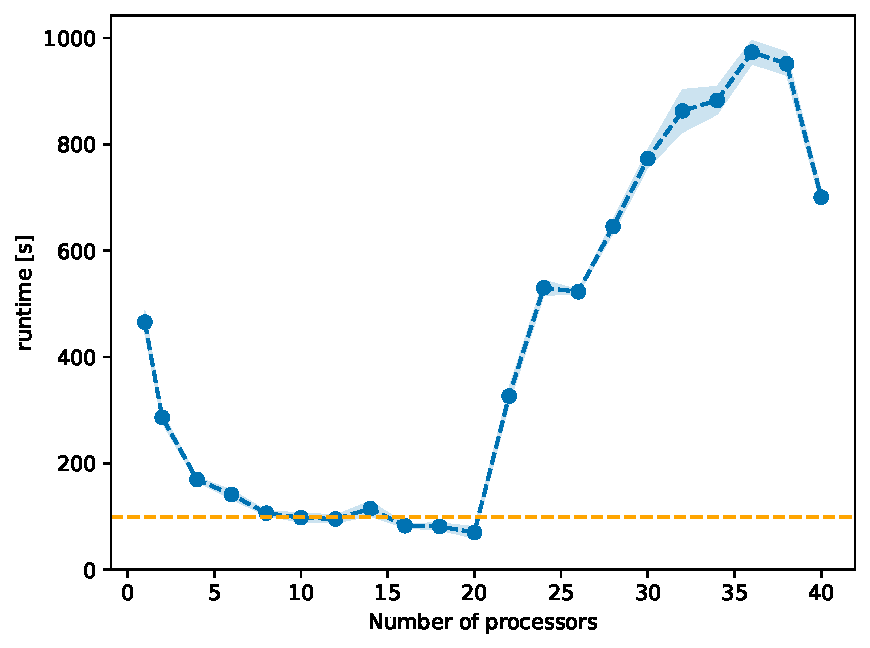
\includegraphics[width=\textwidth]{plots_scf/si_ompi_bench_nprocs_absolute.pdf}
    \subcaption{\gls{openmpi} 4.1.0}
\end{subfigure}
\begin{subfigure}[b]{0.49\textwidth}
    \centering
    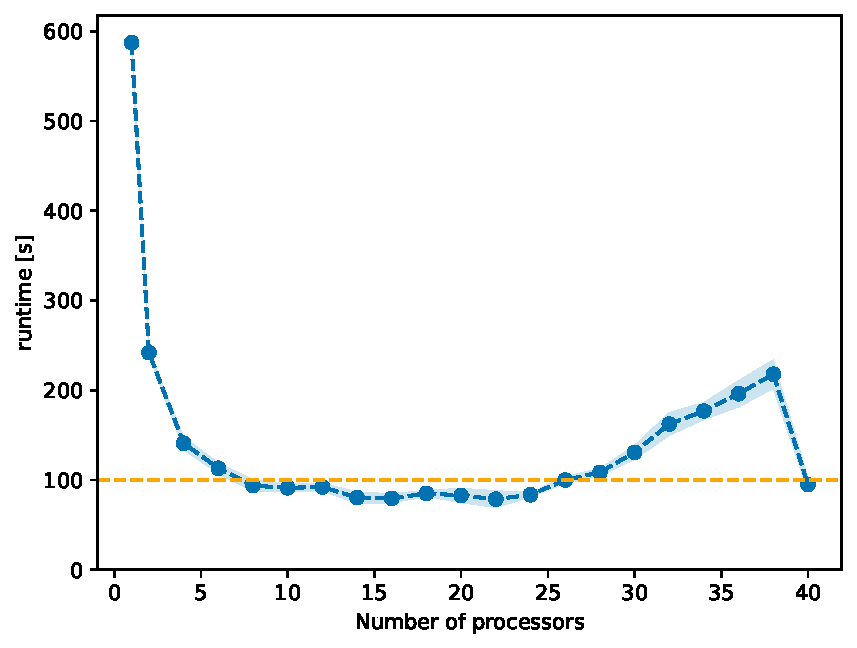
\includegraphics[width=\textwidth]{plots_scf/si_intel_bench_nprocs_absolute.pdf}
    \subcaption{\gls{oneapi} 2021.4}
\end{subfigure}
\caption{Comparison of absolute runtimes between \QE compiled with \gls{openmpi} and \gls{oneapi} for the Si benchmarking system, \emph{\texttt{nk 1} and \texttt{nd 1}}}
\label{fig:scaling_scf_compilers_runtime_si}
\end{figure}
Fig. \ref{fig:scaling_scf_runtime_compilers_nprocs} shows the absolute runtime for both the \gls{openmpi} and \gls{oneapi} benchmarks.
This explains the difference in scaling seen in the speedup plots: the runtime on a single core is significantly higher for the \gls{oneapi} benchmark, so even though the runtime between both benchmarks is about the same starting from around 10 processors there is a difference in speedup.
To assess this more quantitatively, tab. \ref{tab:runtimes_si_scf_compilers} lists the average runtime for some selected number of processors.
Importantly, the runtime for the \gls{oneapi} benchmark is faster for smaller numbers of processors (except 1), but only \SI{15}{\percent} for 2 cores and even smaller differences for more cores, with the \gls{openmpi} calculation being even a little faster for 20 processors.

\begin{table}[ht!]
    \caption{Selected absolute runtimes of \QE compiled with \gls{openmpi} 4.1.0 and \gls{oneapi} 2021.4 for the Si benchmarking system, \emph{\texttt{nk 1} and \texttt{nd 1}}}
    \label{tab:runtimes_si_scf_compilers}
    \begin{tabular}{@{}lll@{}}
    \toprule
    \begin{tabular}[c]{@{}l@{}}Number of\\ processors\end{tabular} & \gls{openmpi} & \gls{oneapi}  \\ \midrule
    1                                                              & \SI{466}{\s}  & \SI{587}{\s}  \\
    2                                                              & \SI{286}{\s}  & \SI{242}{\s}  \\
    4                                                              & \SI{170}{\s}  & \SI{141}{\s}  \\
    10                                                             & \SI{97.9}{\s} & \SI{91.3}{\s} \\
    20                                                             & \SI{70.2}{\s} & \SI{82.8}{\s} \\ \bottomrule
    \end{tabular}
\end{table}

The same benchmark with the \gls{oneapi} compiled version of \QE is shown in fig. \ref{fig:scaling_scf_intel_nprocs_tas2_speedup}.
\begin{figure}[ht!]
    \centering
    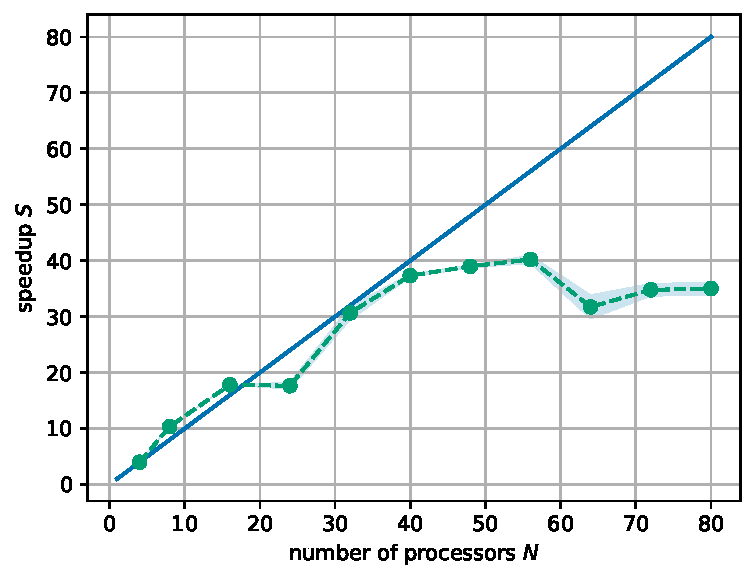
\includegraphics[width=0.75\textwidth]{plots_scf/TaS2_intel_bench_nprocs_speedup.pdf}
    \caption{Scalability for the \TaS benchmarking system, \emph{\QE 7.0 compiled with \gls{oneapi} 2021.4, \texttt{nk 1} and \texttt{nd 1}}}
    \label{fig:scaling_scf_intel_nprocs_tas2_speedup}
\end{figure}

For this system, the speedup follows Amdahl's law, discussed in sec. \ref{sub:scalability_general} with a linear growth in speedup up to 32 processors with a saturation and only a small gain in speedup with more processors.
In contrast to the benchmark with just \gls{openmpi} (fig. \ref{fig:scaling_scf_ompi_nprocs_tas2_speedup}) there is no drop in speedup after 20 processors.

\begin{figure}[ht!]
    \begin{subfigure}[b]{0.49\textwidth}
        \centering
        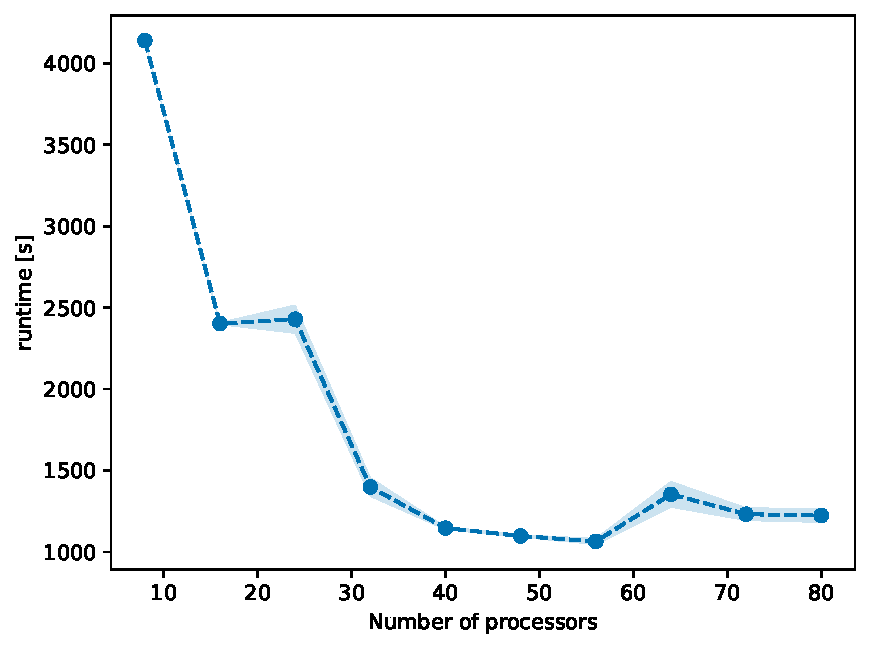
\includegraphics[width=\textwidth]{plots_scf/TaS2_intel_bench_nprocs_absolute.pdf}
    \end{subfigure}
    \begin{subfigure}[b]{0.49\textwidth}
        \centering
        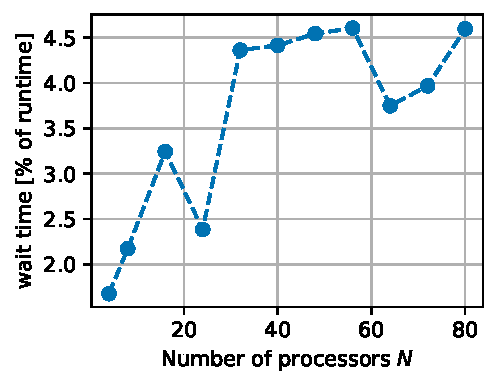
\includegraphics[width=\textwidth]{plots_scf/TaS2_intel_bench_nprocs_wait.pdf}
    \end{subfigure}
    \caption{Absolute runtime and wait time for the scalability test on the \TaS benchmarking system, \emph{\QE compiled with \gls{oneapi} 2021.4, \texttt{nk 1} and \texttt{nd 1}}}
    \label{fig:scaling_scf_intel_nprocs_tas2_absolute_wait}
\end{figure}
Moreover, the absolute runtime shown in fig. \ref{fig:scaling_scf_intel_nprocs_tas2_absolute_wait} 

\todo{TaS2 intel scaling}

This result not only stands for itself as a statement about scaling on a single node, but also provides a basis for scaling beyond the respective optimal ranges of processors for both systems:
The k point parallelization explained in sec. \ref{sub:qe_parallelization} can distribute the workload in such a way that processor pools of sizes within this range work on individual k points and as such can provide optimal scaling within one pool while also not losing performance because the pools do not need to communicate with each other in the same order of magnitude as the pools have to communicate within themselves.
Keeping the results of this section in mind, at least an for the quality k point parallelization can already be made:
For the silicon system, the size of pools should be bigger than 6 processors for optimal scaling and for the \TaS system they should not be bigger than 32 processors.

\section{Using the parallelization parameters of \QE}

\todo{already spoke about k point in the last section, maybe have a better transition here?}
As detailed in section \ref{sub:qe_parallelization}, \QE offers ways to manage how the workload is distributed among the processors.
In \texttt{pw.x} the default plane wave parallelization, k-point-parallelization and linear-algebra parallelization are implemented.

\subsection{k point parallelization}\label{sub:scf_scaling_k_point}

The benchmark pictured in \ref{fig:scaling_scf_nk_si} is set up as follows: for a given number of processors \(N_p\), the parameter \(N_k\) splits the \(N_p\) processors into \(N_k\) processors pools.
As the number of processors in one pool has to be a whole number, only certain combinations of \(N_p\) and \(N_k\) are possible, for example \(N_p = 32\) could be split into processor pools of size 2 with \(N_k = 16\), size 8 with \(N_k = 4\) or size 16 with \(N_k = 2\).
This leads to choosing the size of the processor pools as a variable, not the parameter \texttt{nk}.

Fig. \ref{fig:scaling_scf_nk_si} shows the scaling for poolsizes 2, 8 and 16 for \QE being compiled with OpenMPI/Scalapack and Intel oneAPI.

\begin{figure}[ht!]
\begin{subfigure}[b]{0.49\textwidth}
    \centering
    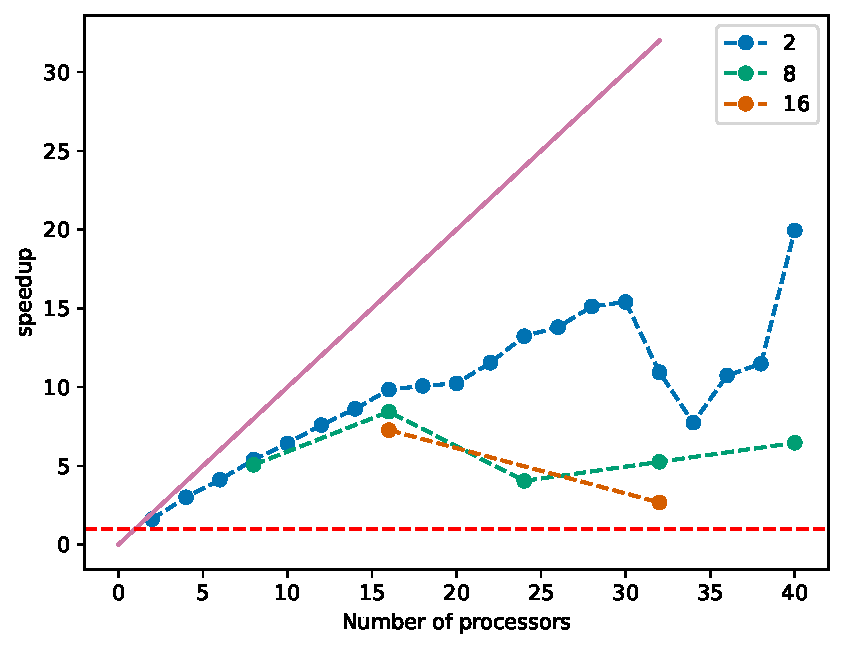
\includegraphics[width=\textwidth]{plots_scf/si_ompi_bench_nk_speedup.pdf}
    \subcaption{\gls{openmpi} 4.1.0}
\end{subfigure}
\begin{subfigure}[b]{0.49\textwidth}
    \centering
    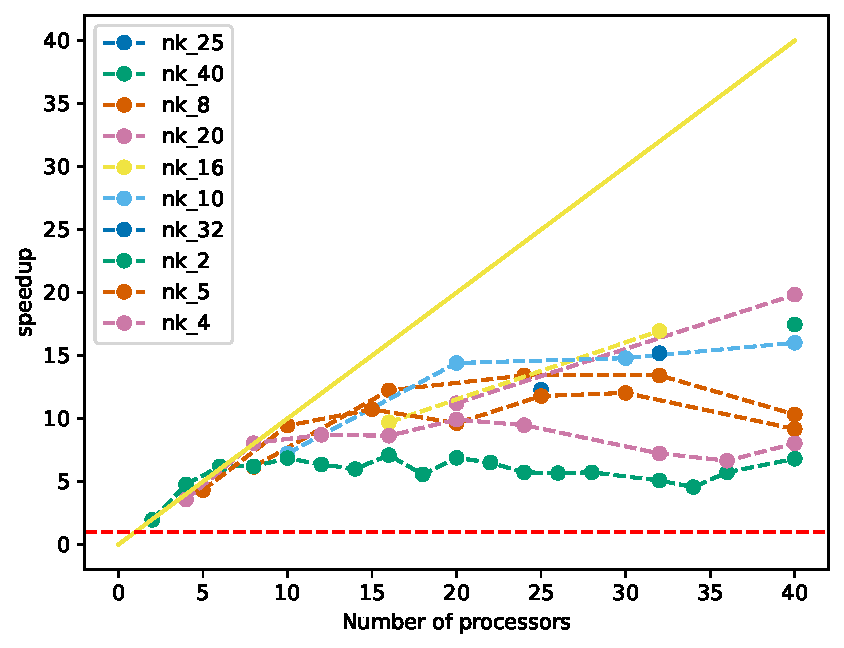
\includegraphics[width=\textwidth]{plots_scf/si_intel_bench_nk_speedup.pdf}
    \subcaption{\gls{oneapi} 2021.4}
\end{subfigure}
\caption{Scalability utilizing k-point parallelization for the Si benchmarking system with 3 different sizes of processor pools. The size is determined by the parameter \texttt{nk} via \emph{size of pools = number of processors / nk}}
\label{fig:scaling_scf_nk_si}
\end{figure}

Fig. \ref{fig:scaling_scf_nk_si} shows that using k parallelization with a pool size of 2 significantly improves the scaling behavior, not only on one node, but especially over more than one node.

\todo{more analysis: difference between poolsizes}

%Another important conclusion to draw out of fig. \ref{fig:scaling_scf_nk_si} is the impact of using Intels compiler instead of OpenMPI, as that factor alone speeds up the calculation by a factor of 2 over the whole range of processors.

\begin{figure}[ht!]
\begin{subfigure}[b]{0.49\textwidth}
    \centering
    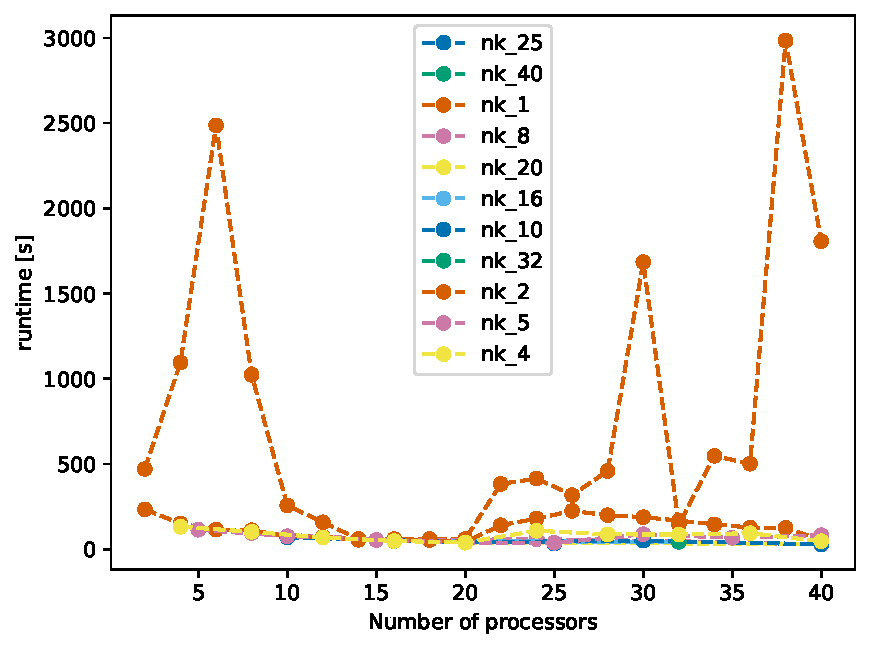
\includegraphics[width=\textwidth]{plots_scf/si_ompi_bench_nk_absolute.pdf}
    \subcaption{\gls{openmpi} 4.1.0}
\end{subfigure}
\begin{subfigure}[b]{0.49\textwidth}
    \centering
    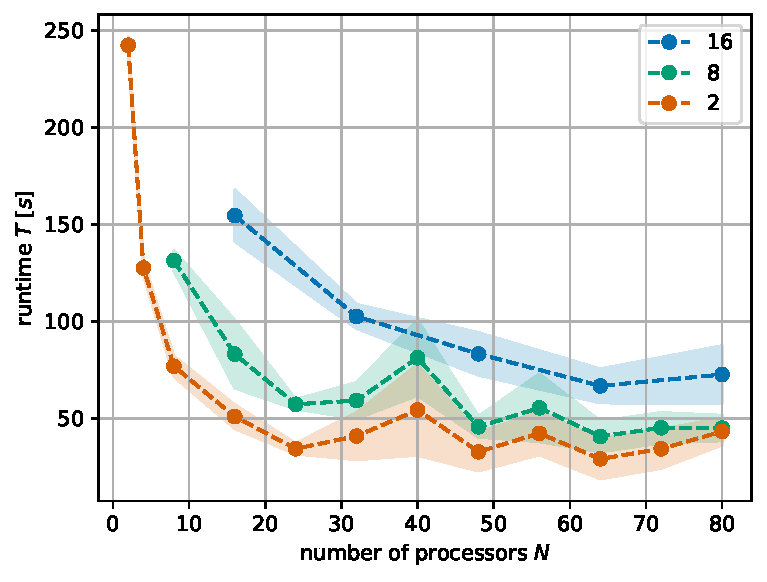
\includegraphics[width=\textwidth]{plots_scf/si_intel_bench_nk_absolute.pdf}
    \subcaption{\gls{oneapi} 2021.4}
\end{subfigure}
\caption{Absolute runtime for the scalability test with k-point parallelization for the Si benchmarking system with 3 different sizes of processor pools, \emph{\texttt{nd 1}}}
\label{fig:scaling_scf_nk_si_absolute}
\end{figure}

\todo{analyse absolute runtimes}

The same scaling test is applied to the \TaS system in fig. \ref{fig:scaling_scf_nk_tas2}.
\begin{figure}[ht!]
    \centering
    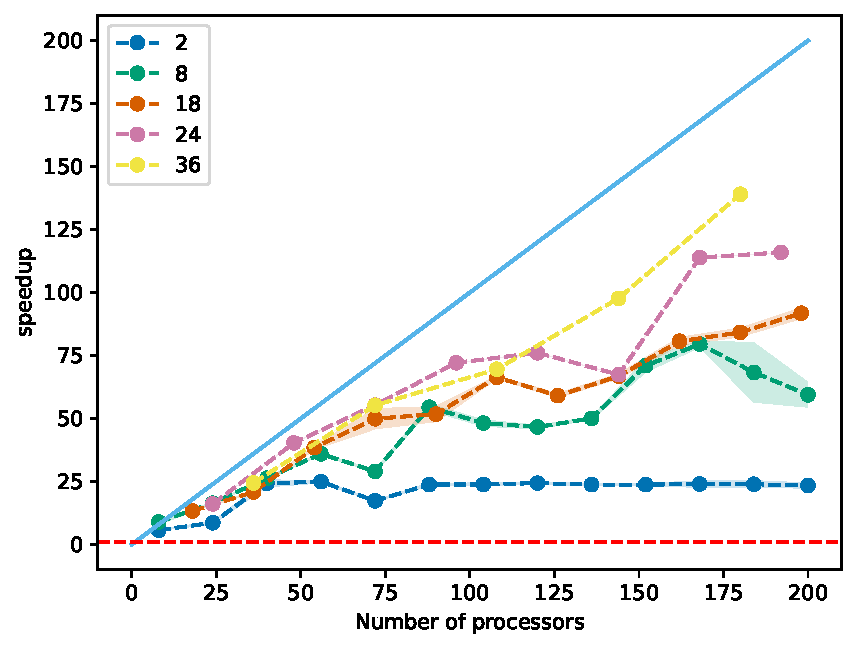
\includegraphics[width=0.8\textwidth]{plots_scf/TaS2_intel_bench_nk_speedup.pdf}
    \caption{Scalability utilizing k-point parallelization for the \TaS benchmarking system over a range of processor pools, \emph{\QE compiled with \gls{oneapi} 2021.4, \texttt{nd 1}}}
    \label{fig:scaling_scf_nk_tas2}
\end{figure}

Remarkably, the scaling behavior is swapped in comparison to fig. \ref{fig:scaling_scf_nk_si}, as the pool size 2 saturates and the bigger pool sizes show way better scaling behavior.
As already alluded to in sec. \ref{sec:scf_scaling_compilers}, the calculations on the \TaS system profit more from parallelization and as such scale better for bigger pool sizes up until 36 processors in one pool, which is the upper limit established in the benchmark just over the number of processors.


It can also be instructive to look at the idle time for this benchmark to judge the quality of parallelization. 
\begin{figure}[ht!]
    \begin{subfigure}[b]{0.49\textwidth}
        \centering
        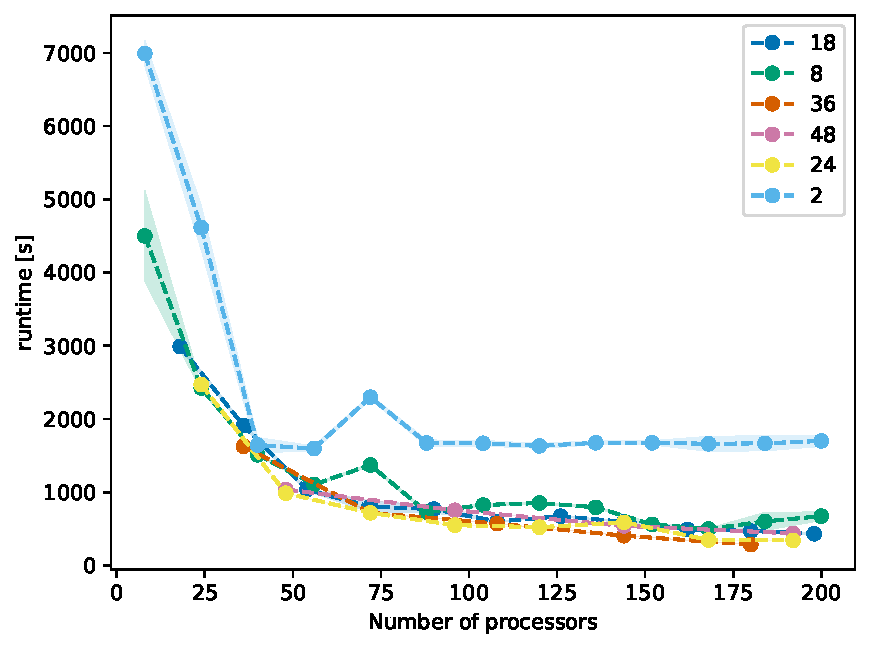
\includegraphics[width=\textwidth]{plots_scf/TaS2_intel_bench_nk_absolute.pdf}
    \end{subfigure}
    \begin{subfigure}[b]{0.49\textwidth}
        \centering
        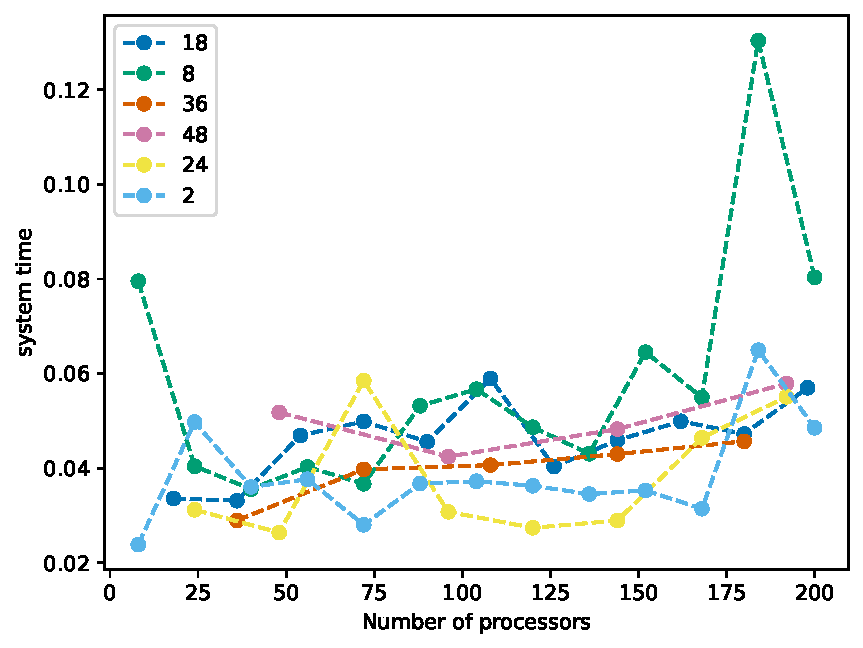
\includegraphics[width=\textwidth]{plots_scf/TaS2_intel_bench_nk_wait.pdf}
    \end{subfigure}
    \caption{Absolute runtime and wait time for the scalability test with k-point parallelization for the \TaS benchmarking system over a range of processor pools, \emph{\QE compiled with \gls{oneapi} 2021.4, \texttt{nd 1}}}
    \label{fig:scaling_scf_nk_tas2_absolute_wait}
\end{figure}


Fig. \ref{fig:scaling_scf_nk_tas2_wait} shows a distribution of idle times between about \(\SI{4}{\percent}\) and \(\SI{6}{\percent}\) of the whole \gls{wall_time}, without any kind of systemic increase over any range of processors.
%This means the parallelization is as good as possible for these 
\todo{more analysis: difference between poolsizes}

\subsection{Linear algebra parallelization}

Fig. \ref{fig:scaling_scf_nd_si} shows the scaling behavior for different values of the parameter \texttt{nd}.
Here, nd\_auto means that no value for \texttt{nd} is specified so \QE automatically chooses the biggest square number smaller than the number of processors.
\begin{figure}[ht!]
\begin{subfigure}[b]{0.49\textwidth}
    \centering
    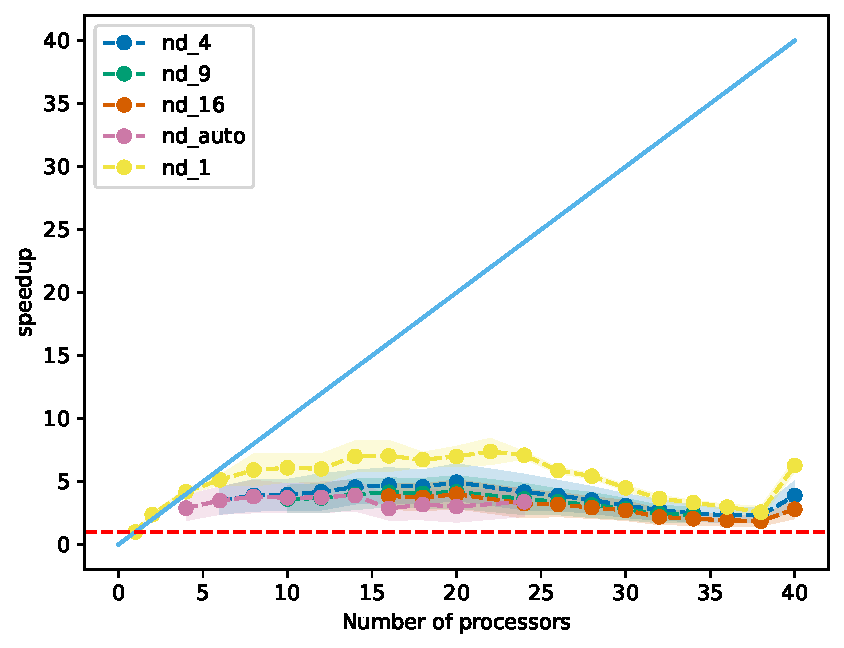
\includegraphics[width=\textwidth]{plots_scf/si_intel_mkl_bench_speedup.pdf}
\end{subfigure}
\begin{subfigure}[b]{0.49\textwidth}
    \centering
    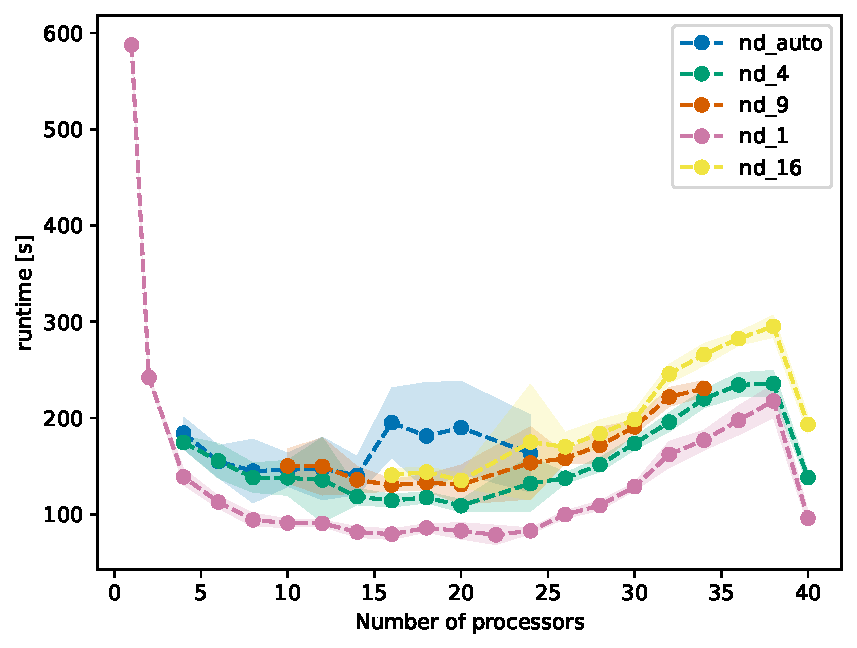
\includegraphics[width=\textwidth]{plots_scf/si_intel_mkl_bench_absolute.pdf}
\end{subfigure}
\label{fig:scaling_scf_nd_si}
\caption{Scalability and runtime utilizing linear algebra parallelization for the Si benchmarking system, \emph{\QE compiled with \gls{oneapi} 2021.4, \texttt{nk 1}}}
\end{figure}
It is clearly shown that using linear algebra parallelization slows the calculation down significantly for the silicon system.

\begin{figure}[ht!]
\begin{subfigure}[b]{0.49\textwidth}
    \centering
    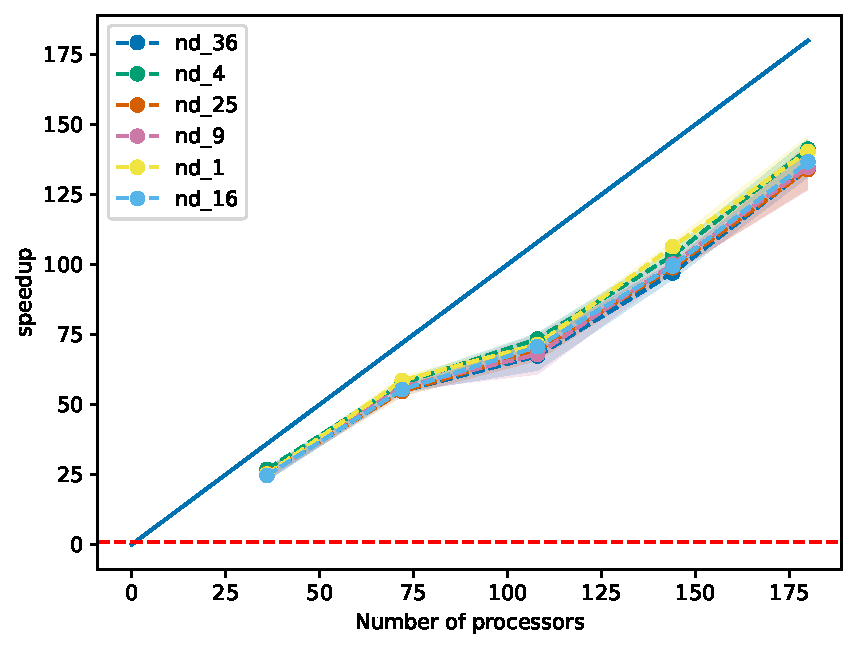
\includegraphics[width=\textwidth]{plots_scf/TaS2_intel_la_parallel_bench_speedup.pdf}
\end{subfigure}
\begin{subfigure}[b]{0.49\textwidth}
    \centering
    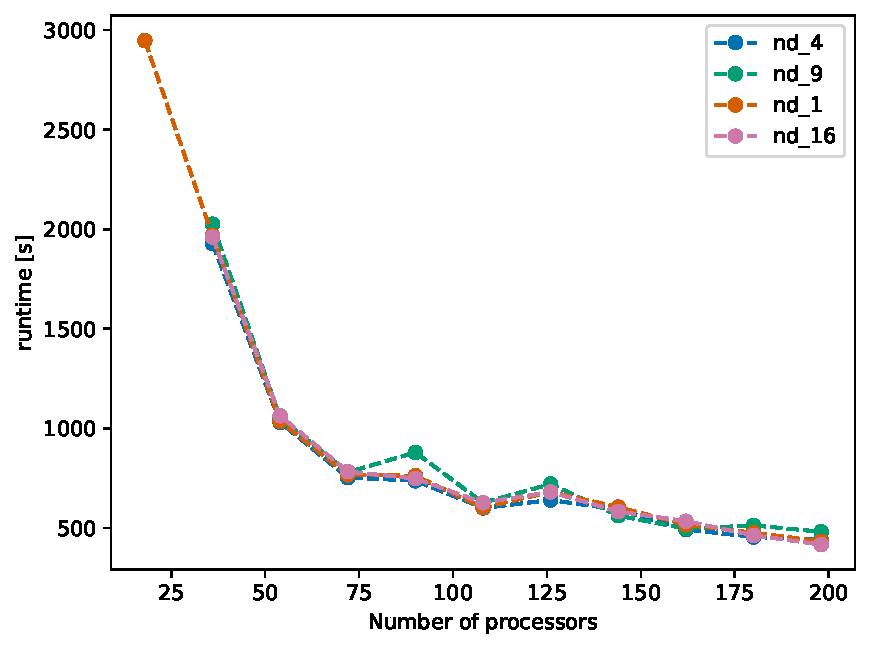
\includegraphics[width=\textwidth]{plots_scf/TaS2_intel_la_parallel_bench_absolute.pdf}
\end{subfigure}
\label{fig:scaling_scf_nd_tas2}
\caption{Scalability and runtime utilizing linear algebra parallelization for the \TaS benchmarking system, \emph{\QE compiled with \gls{oneapi} 2021.4, \texttt{nk} chosen such that pool size = 36}}
\end{figure}

Interestingly, this again is not reproduced for the more expensive \TaS benchmarking system.
Fig. \ref{fig:scaling_scf_nd_tas2} shows a pretty much consistent times across all values for \texttt{nd}.

Those results are already hinted at in the \texttt{PWscf} user guide \cite{noauthor_pwscf_nodate}.
Here, in the guide for choosing parallelization parameters, using linear algebra parallelization is recommended when the number of \acrshort{kohn_sham} states is a few hundred or more.
The silicon system has 8 electrons and is as such described with 4 \gls{kohn_sham} states, the \TaS system has 153 electrons, so \QE uses 92 \gls{kohn_sham} states (in case of metallic materials, the band occupation is smeared around the Fermi energy to avoid level crossings, so more \gls{kohn_sham} states than \(\frac{1}{2} * (\textrm{number of electrons})\) are needed to account for that).
Evidently, this number of \acrshort{kohn_sham} states is on the edge of linear algebra parallelization actually speeding up calculations.

\section{Comparison with calculations on the HLRN cluster}

All calculations so far were exclusively run on the PHYSnet cluster and as such are limited by hardware and configuration present in the cluster.
To assess this limitation, the k point benchmarks from sec. \ref{sub:scf_scaling_k_point} were run again on the another cluster, the HLRN cluster in particular.
The North German Supercomputing Alliance (Norddeutscher Verbund für Hoch- und Höchstleistungsrechnen - HLRN) operates a distributed supercomputer system at the Georg-August-Universität Göttingen and the Zuse Institute Berlin.
The current iteration HLRN-IV has nodes with 2 Intel Cascade Lake Platinum 9242 CPUs (48 cores each) and an Omni-Path (Intel proprietary Infiniband competitor) connection between nodes.

Fig. \ref{fig:scaling_scf_hlrn_nk_si_speedup} and \ref{fig:scaling_scf_hlrn_nk_si_absolute_wait} show the benchmarks for the silicon benchmarking system.
\todo{compiler and MPI version HLRN!}

\begin{figure}[ht!]
\centering
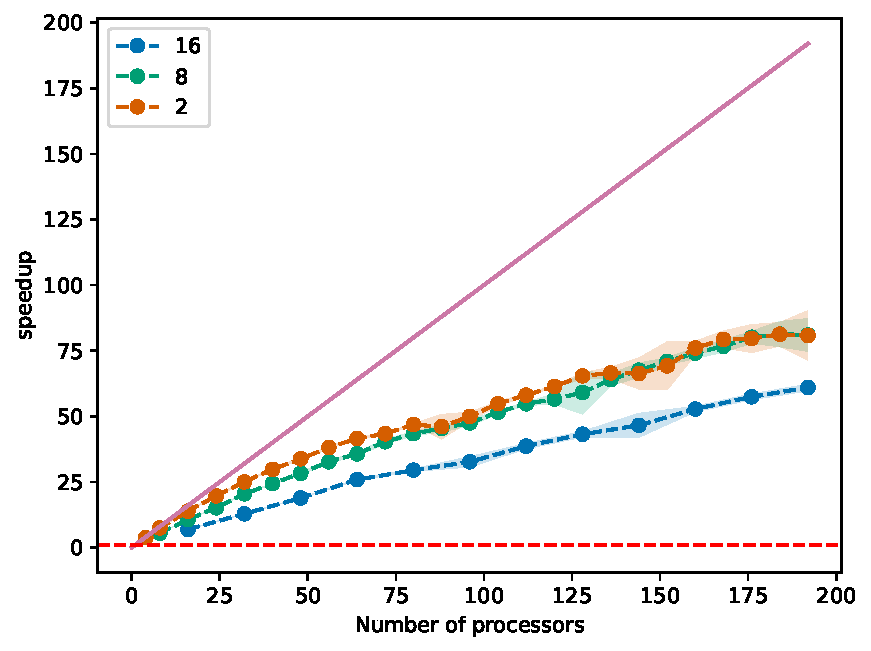
\includegraphics[width=0.75\textwidth]{plots_scf/si_hlrn_bench_nk_speedup.pdf}
\caption{Scalability utilizing k-point parallelization for the Si benchmarking system with 3 different sizes of processor pools run on the HLRN cluster, \emph{\QE compiled with Intel Parallel Studio 2019u5, Intel MPI 2018.5, \texttt{nd 1}}}
\label{fig:scaling_scf_hlrn_nk_si_speedup}
\end{figure}

\begin{figure}[ht!]
\begin{subfigure}[b]{0.49\textwidth}
    \centering
    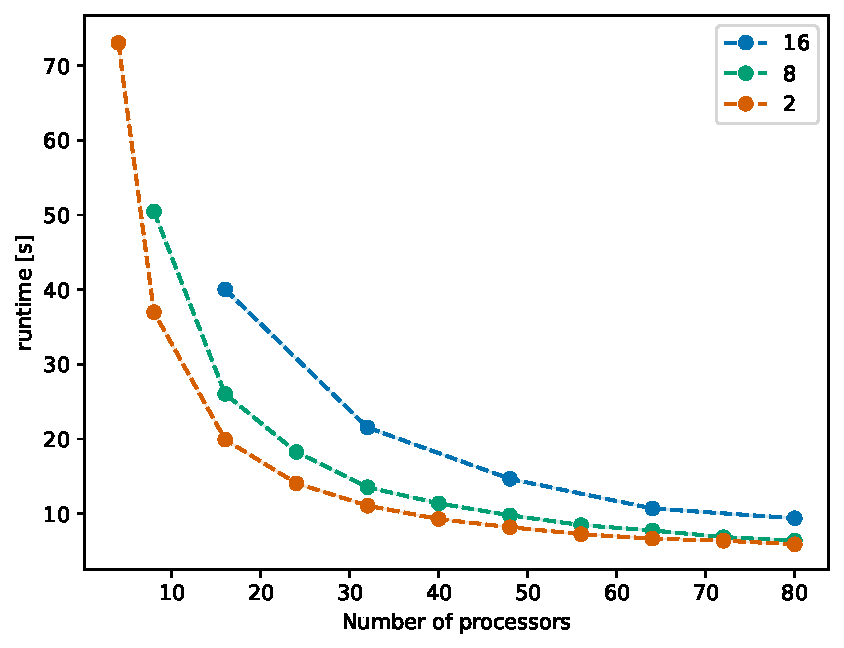
\includegraphics[width=\textwidth]{plots_scf/si_hlrn_bench_nk_absolute.pdf}
\end{subfigure}
\begin{subfigure}[b]{0.49\textwidth}
    \centering
    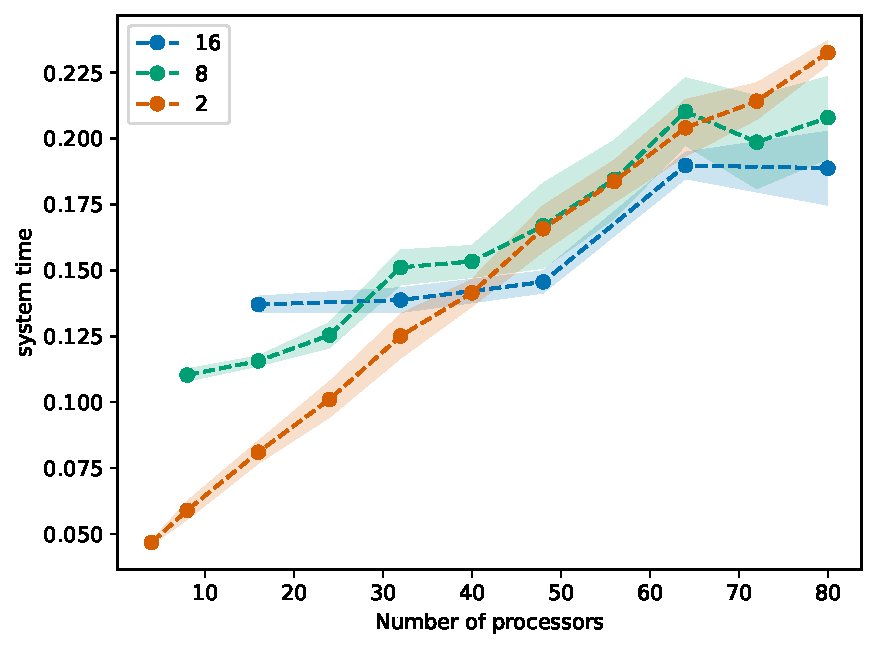
\includegraphics[width=\textwidth]{plots_scf/si_hlrn_bench_nk_wait.pdf}
\end{subfigure}
\caption{Absolute runtime and wait time for the scalability test with k-point parallelization for the Si benchmarking system run on the HLRN cluster, \emph{\QE compiled with Intel Parallel Studio 2019u5, Intel MPI 2018.5, \texttt{nd 1}}}
\label{fig:scaling_scf_hlrn_nk_si_absolute_wait}
\end{figure}
The scaling behavior has some striking differences in comparison with the same benchmarks run on the PHYSnet cluster
First of all, speedup and runtimes are very consistent across runs, with only a minimal variance across the whole range of processors.
This is consistent with the observations made on the PHYSnet, where scaling over a single node also was relatively consistent across runs.


\begin{figure}[ht!]
\centering
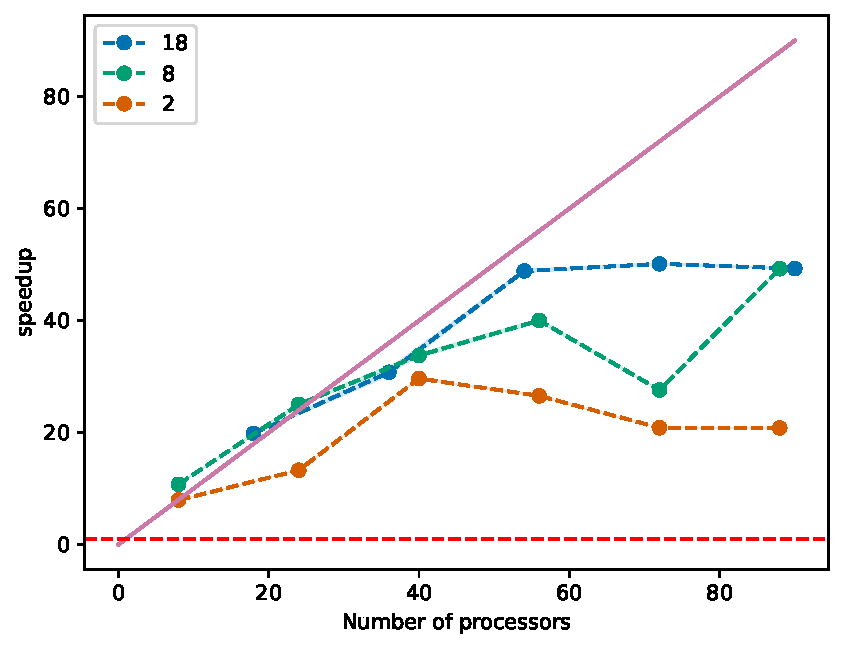
\includegraphics[width=0.75\textwidth]{plots_scf/TaS2_hlrn_bench_nk_speedup.pdf}
\caption{Scalability utilizing k-point parallelization for the \TaS benchmarking system over a range of processor pool sizes run on the HLRN cluster, \emph{\QE compiled with Intel Parallel Studio 2019u5, Intel MPI 2018.5, \texttt{nd 1}}}
\label{fig:scaling_scf_hlrn_nk_TaS2_speedup}
\end{figure}

\begin{figure}[ht!]
\begin{subfigure}[b]{0.49\textwidth}
    \centering
    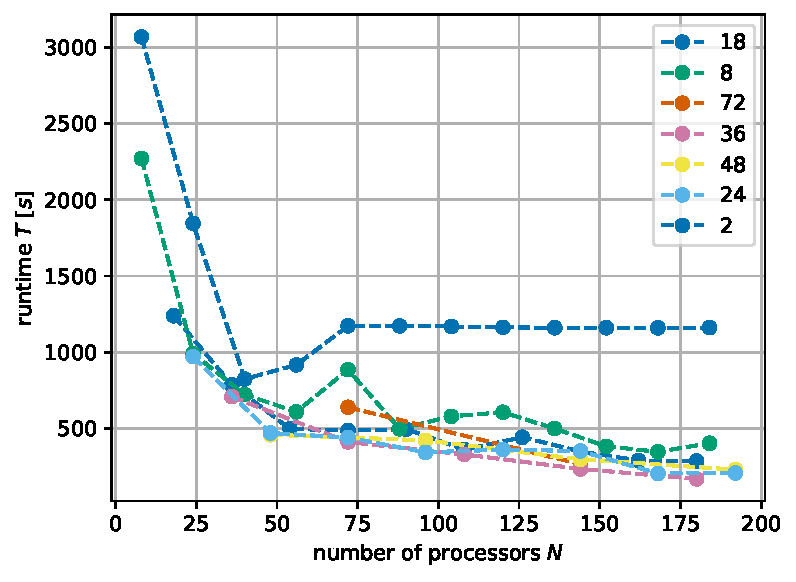
\includegraphics[width=\textwidth]{plots_scf/TaS2_hlrn_bench_nk_absolute.pdf}
\end{subfigure}
\begin{subfigure}[b]{0.49\textwidth}
    \centering
    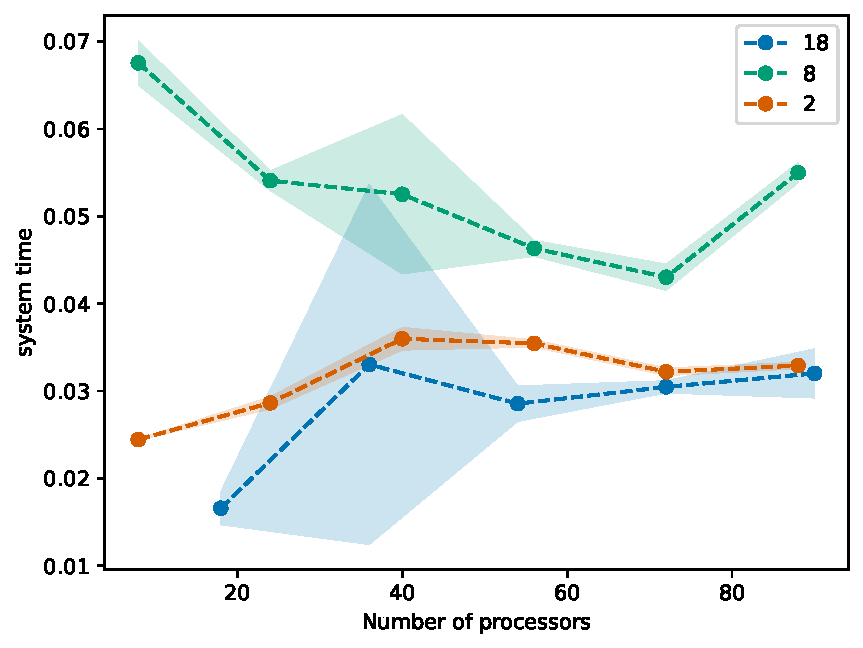
\includegraphics[width=\textwidth]{plots_scf/TaS2_hlrn_bench_nk_wait.pdf}
\end{subfigure}
\caption{Absolute runtime and wait time for the scalability test with k-point parallelization for the \TaS benchmarking system run on the HLRN cluster, \emph{\QE compiled with Intel Parallel Studio 2019u5, Intel MPI 2018.5, \texttt{nd 1}}}
\label{fig:scaling_scf_hlrn_nk_TaS2_absolute_wait}
\end{figure}

\section{Conclusion: Parameters for optimal scaling}

\end{document}